\part{Android knowledge}

\chapter{Android Architecture}


\section{Software Stack}
Android is structured in the form of a software stack comprising applications,
an operating system, run-time environment, middleware, services and
libraries. Each layer of the stack, and the corresponding
elements within each layer, are tightly integrated and carefully tuned to
provide the optimal application development and execution environment for
mobile devices. 

\begin{figure}
    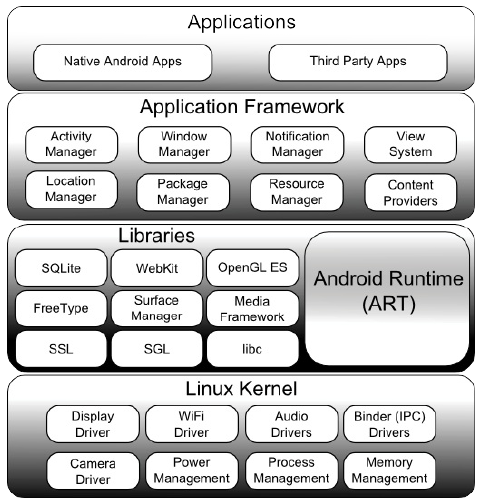
\includegraphics[width=\linewidth]{android_knowledge/os/images/stack.png}
  \caption{Software stack}
  \label{fig:android:sotfware-stack}
\end{figure}


\section{Linux kernel}
 Android uses only the Linux kernel. You can view the Android OS as having two
 distinct sides to it:
\begin{itemize}
    \item a stripped-down and modified Linux kernel 
    \item an application virtual machine that runs Java-like applications.
\end{itemize}

In contrast to conventional Linux computing, each application that is installed
on an Android device is assigned its own unique user identifier (UID) and group
identifier (GID). In certain instances this statement does not hold true and
applications can run under the same user, but these are covered later in this
chapter under the “Application Sandbox” section.

Every Android application has to be given a unique package name by its
developer. The naming convention for these packages should be all lowercase and
the reverse Internet domain name of the organization that developed it
(\verb+com.amazingutils.batterysaver+)

Installed application are assigned a private data directory at the
following location on the  filesystem. 
\begin{verbatim}
shell@android:/ # ls -l /data/data/
...
drwxr-x--x u0_a46 u0_a46 2014-04-10 10:41 com.amazingutils.batterysaver
\end{verbatim}

Notice that the owner of the folder is the newly created user for that
application (\verb+u0_a46+, which translates to \verb+UID 10046+).


\section{Dalvik Virtual Machine (DVM)}
The Dalvik Virtual Machine (DVM) was specifically designed for the Android
platform and is unique to it. The main reason for its existence is that it was
designed to run on hardware with processing and memory constraints and is much
lighter than the normal Java Virtual Machine. It was designed in a way that
allows many Dalvik VMs to be run at the same time in a memory-efficient manner.
The code that runs on it is written and compiled to Java classes and then
converted into a single \verb+DEX+ file using the dx SDK utility. 


\section{Android Runtime (ART)}
When an Android app is built within Android Studio it is compiled into an
intermediate bytecode format (referred to as DEX format). When the
application is subsequently loaded onto the device, the Android Runtime
(ART) uses a process referred to as Ahead-of-Time (AOT) compilation to
translate the bytecode down to the native instructions required by the device
processor. This format is known as Executable and Linkable Format (ELF).

Each time the application is subsequently launched, the ELF executable
version is run, resulting in faster application performance and improved
battery life.

This contrasts with the Just-in-Time (JIT) compilation approach used in
older Android implementations whereby the bytecode was translated within a
virtual machine (VM) each time the application was launched.

\section{Android Libraries}
In addition to a set of standard Java development libraries the Android
development environment also includes the Android Libraries.  A summary of some
key core Android libraries available to the Android developer is as follows:
\begin{itemize}
    \item android.app – Provides access to the application model and is the
        cornerstone of all Android applications.
    \item android.content – Facilitates content access, publishing and
        messaging between applications and application components.a
    \item android.database – Used to access data published by content providers
        and includes SQLite database management classes.
    \item android.graphics – A low-level 2D graphics drawing API including
        colors, points, filters, rectangles and canvases.
    \item android.hardware – Presents an API providing access to hardware such
        as the accelerometer and light sensor.
    \item android.opengl – A Java interface to the OpenGL ES 3D graphics rendering API.
    \item android.os – Provides applications with access to standard operating system services including messages, system services and inter-process communication.
    \item android.media – Provides classes to enable playback of audio and video.
    \item android.net – A set of APIs providing access to the network stack.  Includes android.net.wifi, which provides access to the device’s wireless stack.
    \item android.print – Includes a set of classes that enable content to be sent to configured printers from within Android applications.
    \item android.provider – A set of convenience classes that provide access to standard Android content provider databases such as those maintained by the calendar and contact applications.
    \item android.text – Used to render and manipulate text on a device display.
    \item android.util – A set of utility classes for performing tasks such as string and number conversion, XML handling and date and time manipulation.
    \item android.view – The fundamental building blocks of application user interfaces.
    \item android.widget - A rich collection of pre-built user interface components such as buttons, labels, list views, layout managers, radio buttons etc.
    \item android.webkit – A set of classes intended to allow web-browsing capabilities to be built into applications.
\end{itemize}

It is important to note, however, that the core libraries do not
perform much of the actual work and are, in fact, essentially Java “wrappers”
around a set of C/C++ based libraries.

C/C++ libraries are included to fulfill a wide and diverse range of functions
including 2D and 3D graphics drawing, Secure Sockets Layer (SSL)
communication, SQLite database management, audio and video playback,
bitmap and vector font rendering, display subsystem and graphic layer
management and an implementation of the standard C system library (libc).


In practice, the typical Android application developer will access these
libraries solely through the Java based Android core library APIs. In the event
that direct access to these libraries is needed, this can be achieved using the
Android Native Development Kit (NDK), the purpose of which is to call the
native methods of non-Java or Kotlin programming languages (such as C and
C++) from within Java code using the Java Native Interface (JNI).

\section{Application Framework}
The Application Framework is a set of services that collectively form the
environment in which Android applications run and are managed. This framework
implements the concept that Android applications are constructed from reusable,
interchangeable and replaceable components.  This concept is taken a step
further in that an application is also able to publish its capabilities along
with any corresponding data so that they can be found and reused by other
applications.

The Android framework includes the following key services:

\begin{itemize}
        \item Activity Manager – Controls all aspects of the application
            lifecycle and activity stack.
        \item Content Providers – Allows applications to publish and share data
            with other applications.
        \item Resource Manager – Provides access to non-code embedded resources
            such as strings, color settings and user interface layouts.
        \item Notifications Manager – Allows applications to display alerts and
            notifications to the user.
        \item View System – An extensible set of views used to create
            application user interfaces.
        \item Package Manager – The system by which applications are able to
            find out information about other applications currently installed
            on the device.
        \item Telephony Manager – Provides information to the application about
            the telephony services available on the device such as status and
            subscriber information.
        \item Location Manager – Provides access to the location services
            allowing an application to receive updates about location changes.
\end{itemize}

\section{Applications}
These comprise both the native applications provided with the particular Android
implementation (for example web browser and email applications) and the
third party applications installed by the user after purchasing the device.


\section{Android Applications and Resource Management}

Each running Android application is viewed by the operating system as a
separate process. If the system identifies that resources on the device are
reaching capacity it will take steps to terminate processes to free up memory.

When making a determination as to which process to terminate in order to
free up memory, the system takes into consideration both the priority and
state of all currently running processes, combining these factors to create
what is referred to by Google as an importance hierarchy. Processes are then
terminated starting with the lowest priority and working up the hierarchy 
until sufficient resources have been liberated for the system to function.

\subsection{Android Process States}
Processes host applications and applications are made up of components.
Within an Android system, the current state of a process is defined by the
highest-ranking active component within the application that it hosts. A
process can be in one of the following five states at any given time ordered by
higher to lower priority
\subsubsection{Foreground Process}
These processes are assigned the highest level of priority. At any one time,
there are unlikely to be more than one or two foreground processes active and
these are usually the last to be terminated by the system. A process must meet
one or more of the following criteria to qualify for foreground status:
\begin{itemize}
        \item Hosts an activity with which the user is currently interacting.
        \item Hosts a Service connected to the activity with which the user is interacting.
        \item Hosts a Service that has indicated, via a call to
            \verb+startForeground()+, that termination would be disruptive to the user experience.
        \item Hosts a Service executing either its \verb+onCreate()+,
            \verb+onResume()+ or \verb+onStart()+ callbacks.
        \item Hosts a Broadcast Receiver that is currently executing its
            \verb+onReceive()+ method.
\end{itemize}

\subsubsection{Visible Process}
A process containing an activity that is visible to the user but is not the
activity with which the user is interacting is classified as a “visible process”.
This is typically the case when an activity in the process is visible to the user
but another activity, such as a partial screen or dialog, is in the foreground. A
process is also eligible for visible status if it hosts a Service that is, itself, bound
to a visible or foreground activity.

\subsubsection{Service Process}

Processes that contain a Service that has already been started and is currently
executing.

\subsubsection{Background Process}
A process that contains one or more activities that are not currently visible to
the user, and does not host a Service that qualifies for Service Process status.
Processes that fall into this category are at high risk of termination in the
event that additional memory needs to be freed for higher priority processes.
Android maintains a dynamic list of background processes, terminating
processes in chronological order such that processes that were the least
recently in the foreground are killed first.

\subsubsection{Empty Process}

Empty processes no longer contain any active applications and are held in
memory ready to serve as hosts for newly launched applications. This is
somewhat analogous to keeping the doors open and the engine running on a
bus in anticipation of passengers arriving. Such processes are, obviously,
considered the lowest priority and are the first to be killed to free up
resources.

\subsection{Inter-Process Dependencies}

The situation with regard to determining the highest priority process is
slightly more complex than outlined in the preceding section for the simple
reason that processes can often be inter-dependent. As such, when making a
determination as to the priority of a process, the Android system will also
take into consideration whether the process is in some way serving another
process of higher priority (for example, a service process acting as the content
provider for a foreground process). As a basic rule, the Android
documentation states that a process can never be ranked lower than another
process that it is currently serving.



\chapter{Application}

\section{Anatomy}

\subsection{Activities}
Android applications are created by bringing together one or more components
known as {\bf Activities}.  An activity is a single, standalone module of application
functionality that usually correlates directly to a single user interface
screen and its corresponding functionality. 

Activities are intended as fully reusable and interchangeable building blocks
that can be shared amongst different applications.

Activities are created as subclasses of the Android Activity class and must be
implemented so as to be entirely independent of other activities in the
application. In other words, a shared activity cannot rely on being called at a
known point in a program flow (since other applications may make use of the
activity in unanticipated ways) and one activity cannot directly call methods
or access instance data of another activity. This, instead, is achieved using
{\bf Intents} and {\bf Content Providers}.

By default, an activity cannot return results to the activity from which it was
invoked. If this functionality is required, the activity must be specifically
started as a sub-activity of the originating activity.


All activities must be represented by \verb+<activity>+ elements in the {\bf
manifest file}. Any that are not declared there will not be seen by the system
and will never be run.

The \verb+android:name+ attribute within the \verb+<activity>+ tag specifies
the name of the class that implements that activity.

\begin{verbatim}
<activity 
    android:configChanges="keyboard|keyboardHidden|orientation|screenSize|uiMode" 
    android:label="@string/app_name" 
    android:launchMode="singleTask" 
    android:name="com.routerspace.MainActivity" 
    android:windowSoftInputMode="adjustResize">
        <intent-filter>
            <action android:name="android.intent.action.MAIN"/>
            <category android:name="android.intent.category.LAUNCHER"/>
        </intent-filter>
</activity>
\end{verbatim}

\subsection{Android Intents}
Intents are the mechanism by which one activity is able to launch another and
implement the flow through the activities that make up an application.
Intents consist of a description of the operation to be performed and,
optionally, the data on which it is to be performed.

Intents can be:
\begin{itemize}
        \item {\bf explicit}, in that they request the launch of a specific
            activity by referencing the activity by class name
        \item {\bf implicit} by stating either the type of action to be
            performed or providing data of a specific type on which the action
            is to be performed. 
\end{itemize}

In the case of implicit intents, the Android runtime will select the activity
to launch that most closely matches the criteria specified by the Intent using
a process referred to as {\bf Intent Resolution}.

\subsection{Broadcast Intents}
Broadcast Intent, is a system wide intent that is sent out to all applications
that have registered an “interested” {\bf Broadcast Receiver}. The Android
system, for example, will typically send out Broadcast Intents to indicate
changes in device status such as the completion of system start up, connection
of an external power source to the device or the screen being turned on or
off.

A Broadcast Intent can be:
\begin{itemize}
    \item normal (asynchronous) in that it is sent to all interested Broadcast
        Receivers at more or less the same time
    \item ordered in that it is sent to one receiver at a time where it can be
        processed and then either aborted or allowed to be passed to the next
        Broadcast Receiver.
\end{itemize}

\subsection{Broadcast Receivers}
Broadcast Receivers are the mechanism by which applications are able to
respond to Broadcast Intents. A Broadcast Receiver must be registered by an
application and configured with an {\bf Intent Filter} to indicate the types of
broadcast in which it is interested. When a matching intent is broadcast, the
receiver will be invoked by the Android runtime regardless of whether the
application that registered the receiver is currently running. The receiver then
has 5 seconds in which to complete any tasks required of it before
returning. Broadcast Receivers operate in the background and do not have a
user interface.

\subsection{Android Services}
Android Services are processes that run in the background and do not have a
user interface. They can be started and subsequently managed from activities,
Broadcast Receivers or other Services.

Services can still notify the user of events using notifications and toasts and
are also able to issue Intents.

Services are given a higher priority by the Android runtime than many other
processes and will only be terminated as a last resort by the system in order to
free up resources. In the event that the runtime does need to kill a Service,
however, it will be automatically restarted as soon as adequate resources once
again become available. A Service can reduce the risk of termination by
declaring itself as needing to run in the foreground. This is achieved by
making a call to i\verb+startForeground()+. 

Example situations where a Service might be a practical solution include, as
previously mentioned, the streaming of audio that should continue when the
application is no longer active, or a stock market tracking application that
needs to notify the user when a share hits a specified price.

\subsection{Content Providers}
Content Providers implement a mechanism for the sharing of data between
applications. Any application can provide other applications with access to its
underlying data through the implementation of a Content Provider including
the ability to add, remove and query the data (subject to permissions). Access
to the data is provided via a URI defined by
the Content Provider. Data can be shared in the form of a file or an entire
SQLite database.

The Content Providers currently available on an Android system may be
located using a {\bf Content Resolver}.

\subsubsection{The Application Manifest}
The glue that pulls together the various elements that comprise an application
is the Application Manifest file. It is within this XML based file that the
application outlines the activities, services, broadcast receivers, data providers
and permissions that make up the complete application.

\subsection{Application Resources}

In addition to the manifest file and the Dex files that contain the byte code, an
Android application package will also typically contain a collection of
resource files. These files contain resources such as the strings, images, fonts
and colors that appear in the user interface together with the XML
representation of the user interface layouts. By default, these files are stored in
the \verb+/res+ sub-directory of the application project’s hierarchy.

\subsection{Application Context}
When an application is compiled, a class named \verb+R+ is created that contains
references to the application resources. The application manifest file and
these resources combine to create what is known as the Application Context.
This context, represented by the Android Context class, may be used in the
application code to gain access to the application resources at runtime. In
addition, a wide range of methods may be called on an application’s context
to gather information and make changes to the application’s environment at
runtime.


\section{Android Packages}
An Android package is a bundle that gets installed on an Android device to
provide a new application.

When you unzip an APK you see the final product of all steps listed above. Note
also that a very strictly defined folder structure is used by every APK. The
following is a high-level look at this folder structure:
\begin{verbatim}
/assets
/res
/lib
/META-INF
AndroidManifest.xml
classes.dex
resources.asrc
\end{verbatim}

\begin{itemize}
    \item Assets: Allows the developer to place files in this directory that
            they would like bundled with the application.
   \item Res: Contains all the application activity layouts, images used,
            and any other files that the developer would like accessed from
            code in a structured way. These files are placed in the raw/
            subdirectory.
    \item Lib: Contains any native libraries that are bundled with the
            application. These are split by architecture under this directory
            and loaded by the application according to the detected CPU
            architecture; for example, x86, ARM, MIPS.
    \item META-INF: This folder contains the certificate of the application
            and files that hold an inventory list of all included files in the
            zip archive and their hashes. 
    \item classes.dex: this is essentially the executable file containing
            the Dalvik bytecode of the application. It is the actual code that
            will run on the Dalvik Virtual Machine.
    \item AndroidManifest.xml: the manifest file containing all
            configuration information about the application and defined
            security parameters. This will be explored in detail later in this
            chapter.
    \item Resources.asrc: Resources can be compiled into this file instead
            of being put into the res folder. Also contains any application
            strings.
\end{itemize}



\subsection{Structure of a Package}
Android applications are distributed in the form of a zipped archive with the
file extension of \verb+.apk+, which stands for Android Package. The official
mime-type of an Android Package is
\verb+application/vnd.android.package-archive+. These packages are nothing more
than zip files containing the relevant compiled application code, resources,
and application metadata required to define a complete application. 


\subsection{Build process}
The build process involves many tools and processes that convert a project into
an Android Application Package (APK) or Android App Bundle (AAB). The build
process is very flexible, so it's useful to understand some of what is
happening under the hood.

 The build process for a typical Android app module, follows these general steps:
 \begin{itemize}
    \item The compilers convert source code into DEX (Dalvik Executable) files,
        which include the bytecode that runs on Android devices, and everything
        else into compiled resources.
    \item  The packager combines the DEX files and compiled resources into an
        APK or AAB, depending on the chosen build target. Before your app can
        be installed onto an Android device or distributed to a store, such as
        Google Play, the APK or AAB must be signed.
    \item The packager signs your APK or AAB using either the debug or release keystore:
        \begin{itemize}
            \item If building a debug version the packager signs the app with
                the debug keystore. Android Studio automatically configures new
                projects with a debug keystore.
            \item If building a release version the packager signs the app with
                the release keystore that need to configured. 
        \end{itemize}
    \item Before generating the final APK, the packager uses the zipalign tool
        to optimize the app to use less memory when running on a device.
\end{itemize}

\url{http://developer.android.com/tools/building/index.html}, an APK is
packaged by performing the following tasks:
\begin{itemize}
    \item An SDK tool named \verb+aapt+ (Android Asset Packaging Tool) converts
        all the XML resource files included in the application to a binary
        form. \verb+R.java+ is also produced by \verb+aapt+ to allow
        referencing of resources from code.
    \item A tool named \verb+aidl+ is used to convert any \verb+.aidl+
        files to \verb+.java+ files containing a converted representation of it using a standard Java interface.
    \item All source code and converted output from \verb+aapt+ and \verb+aidl+
        are compiled into \verb+.class+ files by the Java compiler. This
        requires the \verb+android.jar+ file for your desired API version to be
        in the \verb+CLASSPATH+ environment variable.
    \item The \verb+dx+ utility is used to convert the produced \verb+.class+
        files and any third-party libraries into a single \verb+classes.dex+
        file.
    \item All compiled resources, non-compiled resources (such as images or
        additional executables), and the application DEX file are used by the
        \verb+apkbuilder+ tool to package an APK file. More recent versions of
        the SDK have deprecated the standalone apkbuilder tool and included it
        as a class inside \verb+sdklib.jar+. The APK file is signed with a key
        using the \verb+jarsigner+ utility. It can either be signed by a
        default debug key or if it is going to production, it can be signed
        with your generated release key.  
    \item If it is signed with a release key, the APK must be zip-aligned using
        the \verb+zipalign+ tool, which ensures that the application resources
        are aligned optimally for the way that they will be loaded into memory.
        The benefit of this is that the amount of RAM consumed when running the
        application is reduced
\end{itemize}



\section{Lifecycle}




\section{Permissions}
Permissions add security to system data and
features; you can use predefined permissions, define them yourself, or declare them by
writing appropriate entries in \verb+AndroidManifest.xml+.

\subsection{Permission Types}
Permissions come in several flavors according to the desired protection level.
\begin{itemize}
    \item Dangerous: This level corresponds to high-level security-sensitive
        information. The user will be asked whether they want to allow using
        that permission. Once allowed for an app, the allowance will be saved,
        and the user won’t be asked again until the app gets reinstalled or the
        permission gets explicitly revoked by using the system settings app.
    \item Signature: This level corresponds to extremely high-level
        security-sensitive information. Only apps signed with the same
        certificate as the app defining the permission can acquire it. The
        system will check whether the signatures match and then automatically
        grant the permission.
    \item Special: For a couple of use cases, the system grants access to
        certain system resources only by off-band acquisition methods. Namely,
        for permissions \verb+SYSTEM_ALERT_WINDOW+ and \verb+WRITE_SETTINGS+,
        declaring them in the manifest and call special intents to acquire
        them.  The intent action that  have to used for
        \verb+SYSTEM_ALERT_WINDOW+ is
        \verb+Settings.ACTION_MANAGE_OVERLAY_PERMISSION+, and the one for
        \verb+WRITE_SETTINGS+ is \verb+Settings.ACTION_MANAGE_WRITE_SETTINGS+.
        An app should use these two only if absolutely necessary.
    \item Privileged or System Only: These are for system image apps.
\end{itemize}


Permissions are gathered in permission groups. The idea is that once the user has
accepted a permission request from permission A of group G1, another permission inquiry
for another permission B of the same group G1 is not needed. From a user experience
perspective, permission groups show an effect only if we are talking about Dangerous type
permissions; permission groups for Normal permissions have no impact.





\chapter{misc}

\section{example}
The following is an example of compiling a simple Java JAR for Android without
using an IDE. First, create a file named \verb+Test.java+ with the following content:
\begin{verbatim}
class Test
{
    public static void main(String[] args)
    {
        System.out.println("It works! :D");
    }
}
\end{verbatim}
Issue the following commands that will compile the class to normal Java bytecode, and then use the dx utility to
convert it to a JAR that contains Dalvik-compatible bytecode.
\begin{verbatim}
$ javac Test.java
$ dx –dex –output=test.jar Test.class
\end{verbatim}
The JAR is now compiled and can be pushed to the device and executed using the
\verb+dalvikvm+ or \verb+app_process+
binaries on the device. The arguments provided to these binaries tell the Dalvik VM to look for the class named
Test in \verb+/data/local/tmp/test.jar+ and execute the \verb+main+ function.
\begin{verbatim}
$ adb push test.jar /data/local/tmp
$ adb shell dalvikvm -cp /data/local/tmp/test.jar Test
It works :D
\end{verbatim}

The previous code does not produce a full-fledged, installable application on Android. You must follow Android
package conventions and have the SDK automatically package your code into an installable Android package
that can be deployed onto a device. 

\chapter{links}
\begin{itemize}
    \item \url{https://www.veracode.com/security/android-hacking}

    \item \url{https://github.com/sundaysec/Android-Exploits}

    \item
        \url{https://developer.android.com/guide/topics/manifest/manifest-intro}
    \item
        \url{https://developer.android.com/studio/intro}
\end{itemize}
